\textbf{Solution:}

\begin{table}[H]
    \centering
    \begin{tabular}{|c|c|c|c|c|c|c|c|}
        \hline
        A & B & C & !C$\cdot$B & A \texttt{XOR} (BC) & [(!C$\cdot$B) \texttt{XOR} (A \texttt{XOR} (BC))] & A$\cdot$!C & Output \\
        \hline
        0 & 0 & 0 & 0 & 0 & 0 & 0 & 0 \\
        0 & 0 & 1 & 0 & 0 & 0 & 0 & 0 \\
        0 & 1 & 0 & 1 & 0 & 1 & 0 & 1 \\
        0 & 1 & 1 & 0 & 1 & 1 & 0 & 1 \\
        1 & 0 & 0 & 0 & 1 & 1 & 1 & 1 \\
        1 & 0 & 1 & 0 & 1 & 1 & 0 & 1 \\
        1 & 1 & 0 & 1 & 1 & 0 & 1 & 1 \\
        1 & 1 & 1 & 0 & 0 & 0 & 0 & 0 \\
        \hline
    \end{tabular}
    \caption{Detailed truth table for Output = [(!C$\cdot$B) \texttt{XOR} (A \texttt{XOR} (BC))] + A$\cdot$!C}
    \label{tab:detailed_truth_table}
\end{table}

\noindent
Where:
\begin{itemize}
    \item \texttt{XOR} represents XOR operation
    \item $\cdot$ represents AND operation
    \item + represents OR operation
    \item ! represents NOT operation
\end{itemize}
\noindent
The Output column is calculated as the OR (+) of the two previous columns:
\begin{itemize}
    \item Output = [(!C$\cdot$B) \texttt{XOR} (A \texttt{XOR} (BC))] + A$\cdot$!C
\end{itemize}

\vspace{1cm}

\noindent
Simplified truth table showing only inputs and output:

\begin{figure}[H]
    \centering
    \begin{minipage}{0.45\textwidth}
        \centering
        \begin{tabular}{|c|c|c|c|}
            \hline
            A & B & C & Output \\
            \hline
            0 & 0 & 0 & 0 \\
            0 & 0 & 1 & 0 \\
            0 & 1 & 0 & 1 \\
            0 & 1 & 1 & 1 \\
            1 & 0 & 0 & 1 \\
            1 & 0 & 1 & 1 \\
            1 & 1 & 0 & 1 \\
            1 & 1 & 1 & 0 \\
            \hline
        \end{tabular}
        \caption{Simplified truth table for the Boolean function}
        \label{tab:simplified_truth_table}
    \end{minipage}
    \hfill
    \begin{minipage}{0.45\textwidth}
        \centering
        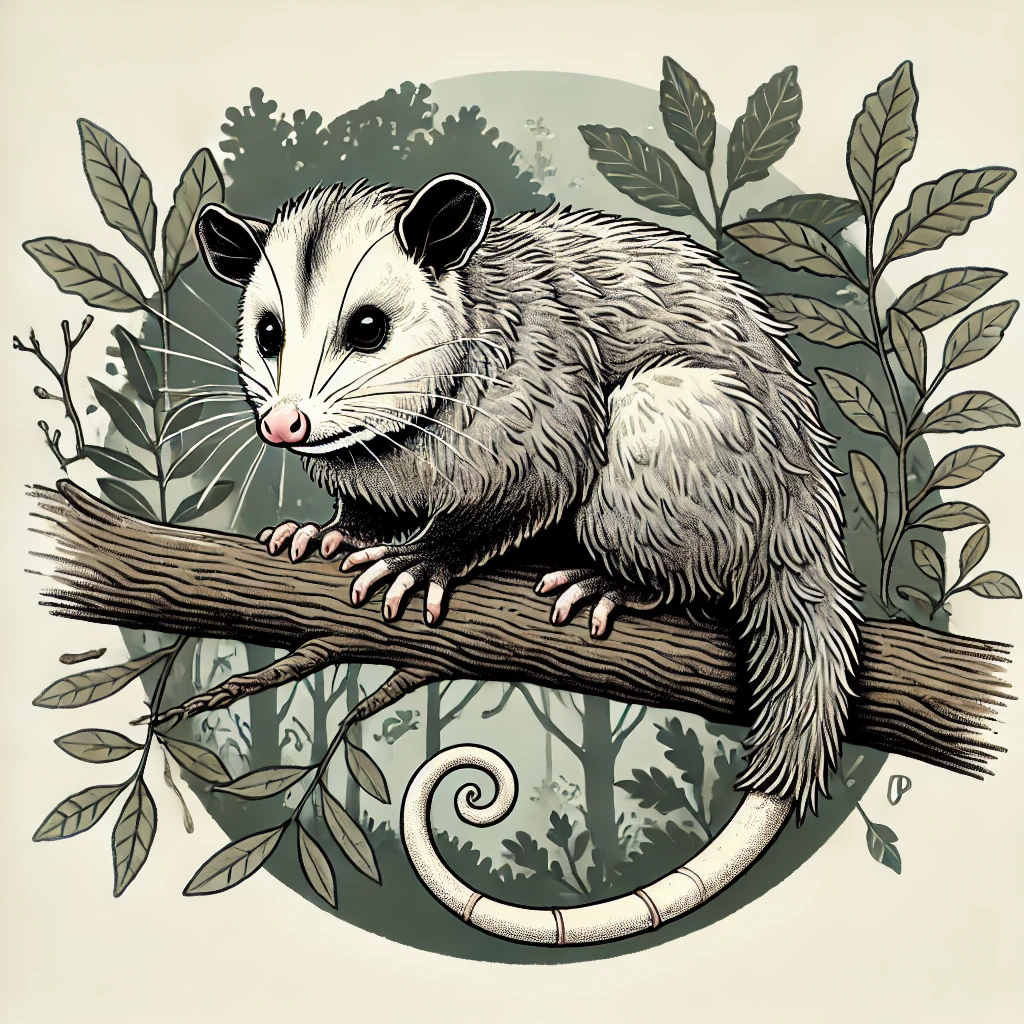
\includegraphics[width=0.62\textwidth]{figures/possum.png}
        \caption{Possum illustration generated using AI (DALL-E)\cite{openai2024possum}}
        \label{fig:possum}
    \end{minipage}
\end{figure}

% ----------------------------------------------------------------
% Drafted by Juntang Wang 2024-10-21
% ----------------------------------------------------------------  
